%----------------------------------------------------------------------------------------
%	PACKAGES AND OTHER DOCUMENT CONFIGURATIONS
%----------------------------------------------------------------------------------------

\documentclass[11pt,fleqn]{book} % Default font size and left-justified equations
\setcounter{secnumdepth}{4}
\setcounter{tocdepth}{4}
\usepackage[top=3cm,bottom=3cm,left=3.2cm,right=3.2cm,headsep=10pt,a4paper]{geometry} % Page margins

\usepackage{xcolor} % Required for specifying colors by name
\definecolor{ocre}{RGB}{243,102,25} % Define the orange color used for highlighting throughout the book

% Font Settings
\usepackage{avant} % Use the Avantgarde font for headings
%\usepackage{times} % Use the Times font for headings
\usepackage{mathptmx} % Use the Adobe Times Roman as the default text font together with math symbols from the Sym­bol, Chancery and Com­puter Modern fonts

\usepackage{microtype} % Slightly tweak font spacing for aesthetics
\usepackage[utf8]{inputenc} % Required for including letters with accents
\usepackage[T1]{fontenc} % Use 8-bit encoding that has 256 glyphs

% Bibliography
\usepackage[style=alphabetic,sorting=nyt,sortcites=true,autopunct=true,babel=hyphen,hyperref=true,abbreviate=false,backref=true,backend=biber]{biblatex}
\addbibresource{bibliography.bib} % BibTeX bibliography file
\defbibheading{bibempty}{}

% Index
\usepackage{calc} % For simpler calculation - used for spacing the index letter headings correctly
\usepackage{makeidx} % Required to make an index
\makeindex % Tells LaTeX to create the files required for indexing
\usepackage{verbatim}
\usepackage{graphicx}
\usepackage{array}
\newcolumntype{L}[1]{>{\raggedright\let\newline\\\arraybackslash\hspace{0pt}}m{#1}}
\usepackage{tabularx}
\newcommand{\source}[1]{\caption*{Source: {#1}} }
%----------------------------------------------------------------------------------------

\begin{document}
	%----------------------------------------------------------------------------------------
	%	TITLE PAGE
	%----------------------------------------------------------------------------------------
	\let\cleardoublepage\clearpage
	\begingroup
	\thispagestyle{empty}
	%\AddToShipoutPicture*{\put(6,5){\includegraphics[scale=1]{portal-energy-background}}} % Image background
	
	\centering

	\par République Tunisienne\\
	Ministère de l'enseignement supérieur\\
	et de la recherche scientifique\\
	Université de Tunis ElManar\par 
	\begin{figure}[!h]
		\begin{center}
			
\includegraphics[width=3cm]{figures/enit}
		\end{center}
	\end{figure}
\textbf{	Département des Technologies de l’Information et de la Communication\\}
	\vspace{1cm}
	\textbf{{\Large Rapport de stage d’ingénieur\\}}
	Groupe: 3ème année Télécommunications\\
	\vspace*{1cm}
	\textbf{{\LARGE Développement Fullstack en Spring et Ionic\\
	Amélioration de l'application Bware\\}}
	\vspace{1cm}
	Réalisé par:\\
	\vspace{0.5cm}
	{\Large Wael ARFAOUI}\\
	\vspace{1cm}
	Entreprise: \textbf{Poulina Group Holding}
	
	\begin{figure}[!h]
		\begin{center}
			
\includegraphics[width=8cm]{figures/poulina}
		\end{center}
	\end{figure}

	Encadré par:\\
	\vspace{0.5cm}
	{\Large Sami BESSAIES\\}
	\vspace{1cm}
	Année Universitaire : 2017-2018
	\par
	
	
	\endgroup
	
	%----------------------------------------------------------------------------------------
	%	Thanks
	%----------------------------------------------------------------------------------------
	\frontmatter
	
	\addcontentsline{toc}{chapter}{Remerciements}
	
	\begin{center}
		\vspace*{5cm}
		\par\normalfont\fontsize{20}{20}\sffamily\selectfont
		Remerciements
		\par\normalfont\fontsize{14}{14}\sffamily\selectfont
		\vspace*{1cm}
		C’est avec plaisir que Nous réservons cette page en signe de gratitude et de profonde reconnaissance à tous ceux qui nous ont aidé à réaliser ce projet.Nous tenons à remercier le jury pour l’honneur qu’il nous a fait pour avoir accepté de juger notre travail. Nous exprimons notre gratitude tout particulièrement à M.Sami Bessaies pour son encadrement, son aide, sa disponibilité, ses conseils fructueux et ses encouragements qu’il nous a prodigué tout au long de ce projet.	Finalement, et avec beaucoup de respect, nous ne pouvons laisser cette occasion sans saluer chaleureusement tous nos enseignants de l’ENIT ainsi que nos collègues pour leur soutien moral.\par
	\end{center}
	
	
	
	%----------------------------------------------------------------------------------------
	%	summary
	%----------------------------------------------------------------------------------------
	\newpage
	\addcontentsline{toc}{chapter}{Résumé}
	\begin{center}
		\vspace*{5cm}
		\normalfont
		{\LARGE Résumé}
		\vspace*{1cm}
	\end{center}
	
	Le présent rapport décrit les différents taches effectuées tout au long de notre expérience comme stagiaire chez Poulina Group Holding. Durant ce stage de trois mois, Nous avons travaillé sur l'application Bware, application développée par Smartdata technology.\\
	Cette application est un moyen de prévention contre les différents problèmes de santé. L'utilisateur peut surveiller tous les risques qui menacent sa santé. Que ce soit la Pollution, le Pollen, la Grippe, la Varicelle ou la Gastro-entérite, Bware" l'informe continuellement du niveau du risque.\\
	
	Le travail demandé consistait à améliorer l'application en rajoutant des fonctionnalités pour les utilisateurs publiques et d'autres pour le suivi et le contrôle de l'application.\\
	
	\textbf{Mots clés} : Santé, Prévention, épidémie, risque, pollution, REST API, Spring Fraework, Ionic framework.\\
	
	
	%----------------------------------------------------------------------------------------
	%	glossary
	%----------------------------------------------------------------------------------------

	\newpage
	\addcontentsline{toc}{chapter}{Glossaire}
	\vspace*{4cm}	
	{\LARGE Glossaire}
	
	\vspace*{1cm}
	\begin{flushleft}
		API Application Programming Interface\\
		CSS Cascading Style Sheet\\
		ENIT Ecole Nationale d’Ingénieurs de Tunis\\
		HTML Hypertext Markup Language\\
		HTTP HyperText Transfer Protocol\\
		JSON JavaScript Object Notation\\
		REST Representational State Transfer\\
		UML Unified Modeling Langage\\
		URI Uniform Resource Identifier\\
	\end{flushleft}

	%----------------------------------------------------------------------------------------
	%	table of contents
	%----------------------------------------------------------------------------------------
	\newpage
	\let\cleardoublepage\clearpage
	\addcontentsline{toc}{chapter}{Liste des figures}
	\renewcommand\listfigurename{Liste des figures}
	\listoffigures
	
	\newpage
	\let\cleardoublepage\clearpage
	\addcontentsline{toc}{chapter}{Liste des tableaux}
	\renewcommand\listtablename{Liste des tableaux} 
	\listoftables
		
	\newpage
	\let\cleardoublepage\clearpage
	\addcontentsline{toc}{chapter}{Table des Matières}
	\renewcommand\contentsname{Table des Matières}
	\tableofcontents
	
	

	
	%----------------------------------------------------------------------------------------
	%	chapters
	%----------------------------------------------------------------------------------------
	\mainmatter
	\addcontentsline{toc}{chapter}{Introduction}
\chapter*{Introduction}
\vspace*{1cm}
\qquad Le monde entier vie sous le rythme d'une évolution et de croissance rapide mais cette croissance vient à un coût cher. Des centaines voire des milliers de menaces contre la santé et l'environnement apparaissent chaque jour.\\

Selon l’Organisation mondiale de la santé (OMS), 3 millions de personnes meurent tous les ans à cause de la pollution de l’air. En 2015, près de 19 milliards d’euros ont été consacrés à des soins de santé lié à la qualité de l’air et 1,2 milliard de journées de travail ont été perdues. Outre les dégâts causés par la pollution de l'air, de nouvelles virus et épidémies apparaissent annuellement contre lesquels l'immunité humaine n'est pas encore développée, ce qui résulte enfin à l'apparition des maladies et des réactions allergiques parfois mortelles.\cite{1}\\

Pour lutter contre les risques présentés ci-dessus la plupart des personnes a recourt aux moyens classiques comme les masques, les gants et les cache-cols pour se protéger contre les différents agents contagieux.\\

L'inconvénient majeur de ces moyens est que les individus sont incapables de savoir au paravent le niveau de pollution ou même l'existence d'un éventuel risque à leur proximité. Et prenant en compte que la météo ne s'intéresse généralement qu'à l'état climatique, les personnes allergiques et fragiles n'ont aucun moyen pour s'informer sur l'état de l'air environnant.\\

La présence d'un moyen d'information sur la qualité quotidienne de l'air s'avère nécessaire surtout pour les personnes fragiles, asthmatiques ou atteintes par une allergie. Un tel outil indiquera le niveau de pollution de l'air en substances nocives, en bactéries et virus ou en pollen. La solution permettra aussi aux utilisateurs de s'inscrire à un type de risque pour recevoir des notifications de suivi ou de conseil. Ainsi une personne inscrite à un risque donné peut suivre les pics de pollution et recevoir en même temps des conseils de protection contre le risque. La solution est une application fiable et pérenne qui permettra de prévenir les utilisateurs de la pollution. Cette dernière fait l’objet de ce rapport où je présente la méthodologie adoptée pour répondre à sa finalité.\\

Le présent rapport décrit les étapes par lesquelles nous avons passé pour finaliser notre projet. Au début, nous présenterons le contexte général de notre application. Dans une deuxième étape, nous analyserons les besoins fonctionnels et non fonctionnels. Le troisième chapitre est consacré aux éléments de conception sur les niveaux : global et détaillé. Enfin nous avons dédié le dernier chapitre pour la réalisation dans laquelle nous présenterons les outils et l’environnement logiciel et matériel utilisés afin de réaliser notre application et nous expliquerons les interfaces de notre projet.


	\chapter{Présentation générale du projet}
\section*{Introduction}
\qquad Nous consacrerons le présent chapitre à la présentation du contexte général de notre Projet, commençant par l’explication de cadre général de projet et son objectif, puis nous attaquerons la partie liée à l’étude de l’existant. Finalement une clarification sur la méthodologie de travail sera entamée.

\section{Cadre du projet}

\qquad Durant notre formation d'ingénieur nous sommes menés à effectuer un stage d'été d'au moins deux mois. Le présent stage a été élaboré à Poulina Group Holding et il consiste à améliorer l'application Bware développée par Smartdata technology.

\subsection{Entreprise d'accueil} 

\qquad Le stage a été effectué au sein de Aster Training filiale du groupe Poulina.

\subsubsection{Poulina Group Holding} 

\qquad Poulina est un groupe industriel et de services tunisien. Originellement spécialisé dans l’agriculture, le groupe s’est peu à peu diversifié pour devenir le premier groupe à capitaux privés du pays.\\

Le groupe s’est organisé au fil des années autour d’une dizaine de métiers regroupant les pôles d’activités de la holding : immobilier, travaux publics, bois et biens d’équipement, produits de grande consommation, emballage, transformation de l’acier, commerce et services, matériaux de construction et intégration avicole.

\subsubsection{Aster Training}

\qquad La société Aster training est une filiale du groupe Poulina et son capital social s’élève à 145000 DT. Créée en 1996, la société Aster training assure les activités suivantes :
\begin{itemize}
	\item Organise des séminaires de formation en gestion, technique et informatique.
	\item Ingénierie informatique.
	\item Étude, conception et développements des logiciels informatiques.
	\item Étude et mise en place des réseaux informatiques.
	\item Infogérance.
	\item Audit et conseil informatiques.
\end{itemize}

\subsection{Objectif du projet}

\qquad Le but du projet est d'apporter des améliorations à l'application Bware développée par l'entreprise française Smart Data Technology. Ces amélioration toucheront la partie destinées aux clients finales, la partie serveur ainsi que la partie destinée au suivi et contrôle de l'application.

\section{Études de l'existant}

\qquad De nos jours, nous témoignons une expansion du marché des applications mobiles. Parmi ces applications on note la présence d'une catégorie destinée à la santé humaine avec un pourcentage de 1\% du marché des applications et qui voit un accroissement d'à peu près 50\% chaque année. Gardant à l'esprit la nécessité cruciale de ces applications pour certains utilisateurs que ce soit pour des raisons de suivi de leur performance physique ou leur état sanitaire (tension, glycémie, température interne ...), nous déduirons en que la catégorie santé et fitness est un marché très important dans le domaine des applications mobiles. Notre intérêt est d'étudier les applications de prévention contre la pollution. Ainsi plusieurs solutions s'offrent aux utilisateurs des mobiles garantissant le suivi du niveau de la pollution à savoir Air Visual, Plume Air Report.

\subsection{Analyse de l'existant}

\qquad Les solutions présentées ci-dessus ne couvrent pas l'intégralité des fonctionnalités nécessaires pour les utilisateurs mais elles en offrent d'autres telles que le partage de l'état de l'air dans les réseaux sociaux et la couverture des villes de partout dans le monde. Parmi les fonctionnalités absentes, nous citons :
\begin{itemize}
	\item Les notifications pour Air Visual
	\item Les détails sur les différents type de pollution pour Plume Air Report
	\item La présence de la carte
\end{itemize} 

\subsection{Critique de l'existant}

\qquad Les exemples cités précédemment ne permettent d'intégrer qu'une partie des fonctionnalités nécessaires pour le suivi du niveaux de la pollution dans des zones éparpillées dans le monde en raison d'une quarantaine de villes par pays. Nous citons aussi d'autres fonctionnalités absentes chez les concurrents telles que les notifications, les conseils et les détails sur les différents type de pollution.

\subsection{Solution proposée}

\qquad Notre solution consiste à couvrir les déficiences des applications présentées en mettant en place une application mobile multiplate-forme destinée aux utilisateurs français qui couvrira la totalité du territoire français mais qui permettra aussi de prévenir les utilisateurs des différents risques auxquels ils sont inscrits, d'afficher des détails sur les agents nocifs et des conseils concernant les niveaux de risque élevés.\\

\section{Méthodologie de travail}

\qquad Pour mener à bien notre projet nous avons opté pour une méthodologie afin d'organiser les différentes phases du projet.\\

Alors nous avons adopté l'approche agile qui consiste à un paradigme révolutionnaire dans le monde de gestion de projet. Cet approche diffère des méthodes classiques par la migration du centre d'intérêt des étapes par lesquels passe le projet vers les étapes par lesquels passe le produit. Ainsi, cet approche élimine l'effet tunnel pour donner davantage de visibilité et de transparence en impliquant le client dans  tous les procès de la réalisation. Ce qui résulte en des majeurs changements sur tout le processus de réalisation qui devient à la fois itératif et incrémental ce qui permettra une meilleure flexibilité aux niveaux de la spécification des besoins mais en gardant un minimum de règles.\\

\subsection{Méthode Scrum}

Au sein de ce cadre méthodologique de gestion de projet, les acteurs ajustent empiriquement, au fil des itérations, leur propre méthode en fonction de leur contexte. On peut qualifier Scrum de simple, pragmatique, transparent et empirique. Scrum ne couvrant que les aspects de gestion de projet, c’est souvent la méthodeeXtreme Programming (XP) qui vient compléter le vide laissé en matière de pratiques de développement. XP apporte ainsi les pratiques de programmation en binôme, de développement piloté par les tests (TDD ou Test Driven Development), intégration continue, etc.\\
Le cycle préconisé par TDD comporte cinq étapes \cite{2}.
   \begin{itemize}
   	\item Écrire un premier test ;
   	\item Vérifier qu’il échoue (car le code qu’il teste n’existe pas), afin de vérifier que le test est valide ;
   	\item Écrire juste le code suffisant pour passer le test ;
   	\item Vérifier que le test passe ;
   	\item Puis ré-usiner le code, c’est-à-dire l’améliorer tout en gardant les mêmes fonctionnalités
   \end{itemize}

\section*{Conclusion}

\qquad Dans ce chapitre, nous avons présenté le cadre général de notre stage en énonçant notre entreprise d’accueil et les objectifs envisagés de ce stage. Nous nous sommes intéressés, par la suite, à l’analyse et la critique des solutions similaires déjà existantes dans le marché et à la proposition de notre solution alternative.

	\chapter{Analyse et spécification des besoins}

\section*{Introduction}

\qquad Après avoir présenté le contexte général de notre projet, nous venons d’énoncer dans cette partie les besoins auxquels notre application devra réponde. Nous énumérerons les besoins fonctionnels et non fonctionnels dans une première partie et nous exposerons par la suite la spécification de ces besoins à travers les diagrammes de cas d’utilisation.

\section{Analyse des besoins}

\qquad Ce chapitre est dédié à l'étude profonde des différents besoins sur l'échelle fonctionnelle et non fonctionnelle. Nous projetons de détailler les risques et contraintes auxquelles est soumis notre projet dans le but de répondre aux besoins.

\subsection{Identification des acteurs}

\qquad L'application doit garantir la prévention contre les risques de pollution pour l'utilisateur final et la suivi et contrôle pour les administrateurs de Smartdata.

\subsection{Besoins fonctionnels}
\qquad Nous présentons ci-dessous les besoins fonctionnels regroupés par acteur:

\begin{itemize}
	\item Utilisateur
		\begin{itemize}
			\item Visualisation des niveaux des risques
			\item Inscription aux différents risques
			\item Visualisation des détails sur les risques
			\item Visualisation des états des stations
			\item Visualisation des conseils
			\item Inscription aux rappels santé
			\item Ajout d'astuces
		\end{itemize}
	\item Administrateur
		\begin{itemize}
			\item Consultation des statistiques
			\item Réception des Emails concernant les batchs
			\item Réception des Emails concernant les notifications
		\end{itemize}
\end{itemize}

\subsection{Besoins non fonctionnels}

\qquad Pour bien répondre à ses besoins notre application doit respecter les exigences techniques suivantes: 

\textbf{Ergonomie} Le but de l’application est qu’elle soit exploitée par des simples utilisateurs qui ne sont pas forcément expérimentés dans le domaine de l’informatique, et qu’elle le soit de la façon la plus efficace. Les interfaces de l’application doivent être ergonomiques et conviviales.

\textbf{Environnement et architecture} L’application doit être mise en place dans une architecture répartie multi-tiers et accessible via le Web à travers les navigateurs Web.

\textbf{Rapidité} Notre application doit garantir un accès rapide aux données et d’une manière transparente.

\textbf{Scalabilité} L’application doit être facilement extensible pour pouvoir accueillir un public plus large.

\textbf{Documentation} L’application sera livrée avec une documentation des différentes fonctions et API qu’elle offre, nécessaire pour les futurs développeur

\section{Spécification des besoins}

\qquad Dans ce paragraphe, nous allons préciser les différents besoins de notre application en ayant recours au langage de modélisations UML. Nous illustrons les besoins par les diagrammes de cas d'utilisation.

\subsection{Diagramme de cas d'utilisation global}

\qquad Nous présentons dans cette partie le diagramme de cas d'utilisation global de notre application. La figure \ref{fig2.1} représente le diagramme de cas d'utilisation global.

\begin{figure}[!h]

	\begin{center}
		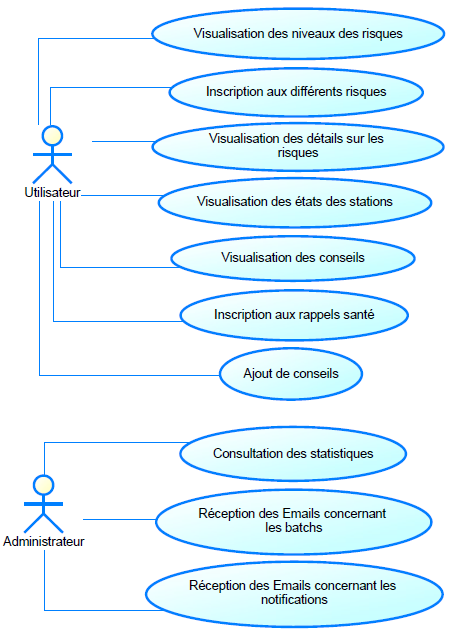
\includegraphics[width =7.1cm ]{figures/globalusecase}		
	\end{center}
	\caption{Diagramme des cas d'utilisation global}
	\label{fig2.1}
\end{figure}

\subsection{Raffinement des cas d'utilisation}

\qquad Dans cette partie, nous présentons les diagrammes de cas d'utilisation raffinés. Nous détaillerons quelques cas d'utilisation parmi ceux qui sont précédemment présentés. 

\subsubsection{Cas d'utilisation : Ajouter astuces}

\qquad La figure \ref{fig2.2} représente le diagramme de cas d'utilisation de l'ajout des astuces.

\begin{figure}[!h]
	\begin{center}
		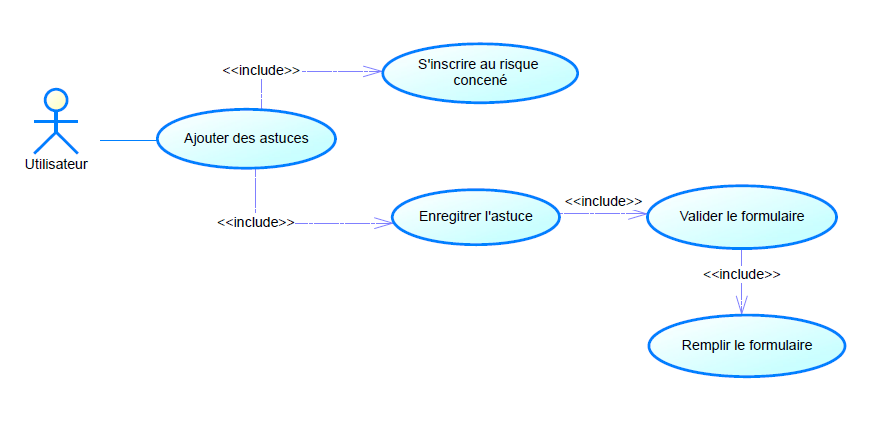
\includegraphics[width=0.64\textheight]{figures/uc_ajoutastuce}
	\end{center}
	\caption{Cas d'utilisation : Ajouter des astuces}
	\label{fig2.2}
\end{figure}

Ci-dessous une description sous forme de tableau du cas d'utilisation : Ajouter astuce.

\begin{table}[!h]
	\caption{Description textuelle du cas d'utilisation : Ajouter astuce}
	\begin{center}
		\begin{tabular}{|L{4cm}|L{10cm}|}
			\hline
			\textbf{Cas d’utilisation} & Ajouter astuce\\
			\hline
			\textbf{Objectif} & Permettre d'ajouter des astuces\\
			\hline
			\textbf{Acteur} & Utilisateur\\
			\hline
			\textbf{Pré-conditions} & S'inscrire, remplir et valider le formulaire\\
			\hline
			\textbf{Post-condition} & Astuce ajoutée\\
			\hline			
			\textbf{Scénarios nominaux} & \textbf{S1. Soumettre une astuce} L'utilisateur remplie le formulaire d'ajout d'astuces, choisit le type de risque, saisit son adresse électronique enfin il confirme l'ajout par cliquer sur le bouton enregistrer\\
			\hline
			\textbf{Exceptions} & \textbf{E1} Utilisateur non inscrit au risque.\\ &\textbf{E2} L'un des champs du formulaire est soit vide soit non valide.\\
			\hline
		\end{tabular}
	\end{center}
\end{table}
 
\subsubsection{Cas d'utilisation : visualisation des niveaux des risques}
\qquad Cette partie est consacrée au raffinement du cas d'utilisation : visualisation des niveaux des risques. La figure \ref{fig2.3} représente en détail le cas d'utilisation avec son acteur et ses pré-conditions.\\

\begin{figure}[!h]
	\begin{center}
		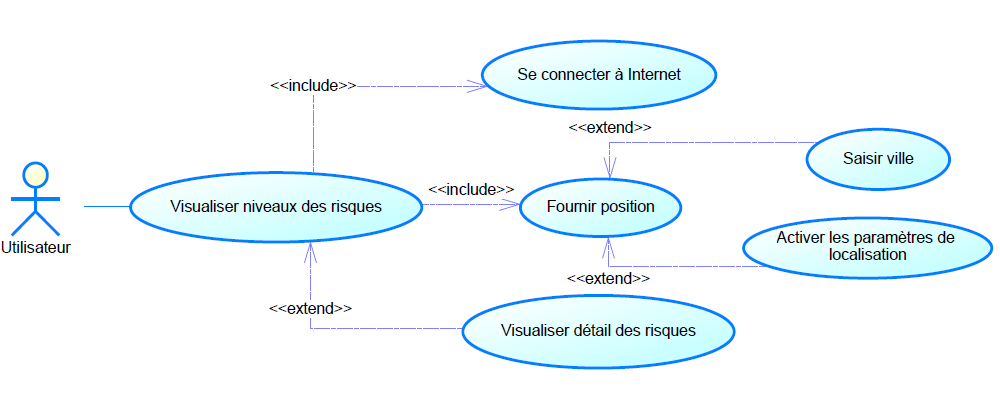
\includegraphics[width=0.64\textheight]{figures/uc_visualisationrisques}
	\end{center}
	\caption{Cas d'utilisation :  visualisation des niveaux des risques}
	\label{fig2.3}
\end{figure}
Le tableau ci-après est une description textuelle du cas d'utilisation.
\begin{table}[!h]
	\caption{Description textuelle du cas d'utilisation : visualiser les niveaux des risques}
	\begin{center}
		\begin{tabular}{|L{4cm}|L{10cm}|}
			\hline
			\textbf{Cas d’utilisation} & visualiser les niveaux des risques\\
			\hline
			\textbf{Objectif} & Permettre de consulter les niveaux des risques\\
			\hline
			\textbf{Acteur} & Utilisateur\\
			\hline
			\textbf{Pré-conditions} & S'inscrire, saisir ville, activer la géolocalisation, se connecter à Internet\\
			\hline
			\textbf{Post-condition} & Niveaux des risques consultés \\
			\hline			
			\textbf{Scénarios nominaux} & \textbf{S1. Consulter le niveau des risques} L'utilisateur se connecte à internet et fournit la ville qu'il veut consulter en saisissant la ville ou en activant le système GPS. Il recevra ainsi le niveaux de risques de la ville souhaitée.\\
			&\textbf{S2} Après avoir reçu les niveaux de risque, l'utilisateur peut consulter les détails sur chaque risque (polluant)\\
			\hline
			\textbf{Exceptions} & \textbf{E1} Utilisateur non inscrit au risque.\\ &\textbf{E2} Téléphone non connecté à Internet\\
			&\textbf{E3} Ville non fourni et système GPS non activé\\
			\hline
		\end{tabular}
	\end{center}
\end{table}
\section*{Conclusion}
\qquad Nous avons consacré ce chapitre, à la spécification des besoins, ce qui permet de mieux comprendre les problématiques soulevées et d’avoir une vue globale sur les fonctionnalités constituantes notre projet. Nous nous intéressons dans le chapitre suivant aux éléments de conception basée sur le travail effectué dans le présent chapitre.
	\chapter{Conception}

\section*{Introduction}
\qquad Dans ce chapitre, nous nous intéressons à la conception de notre projet. En effet la conception s'avère la pierre angulaire de tout projet appelant à l'ingénierie. En se basant sur la spécification détaillée des besoins, nous allons pouvoir définir tout les éléments faisant partie de la réalisation. Nous préciserons alors les éléments de la conception architecturale ainsi ceux de la conception détaillée.\\

\section{Conception globale}

\qquad Nonobstant la simplicité du besoin de notre application, ce dernier n'est pas aussi évident à réaliser car il fait appel à un certain niveau de complexité architecturale. Généralement notre application est composée de deux majeures parties à savoir : la partie Backend, responsable de tous les traitements possibles, la collecte des données et la réponse aux requêtes des clients, et la partie Frontend qui est la partie déployée chez les utilisateurs qui servira comme une Interface Homme Machine (IHM). La figure \ref{fig3.1} illustre l'architecture de notre système. Nous y revenons en plus de détail par la suite.

\begin{figure}[!h]
	\begin{center}
		\includegraphics[width=0.914\linewidth]{figures/arch}
	\end{center}
	\caption{Architecture globale de l'application}
	\label{fig3.1}
\end{figure} 

La communication entre la partie front et back se fait à base de services Web REST (HTTP et JSON). En fait, la partie Frontend consomme les services web fournis par la partie Backend. (Voir figure \ref{fig3.2})

\begin{figure}[!h]
	\begin{center}
		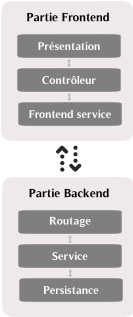
\includegraphics{figures/liaison}
	\end{center}
	\caption{Architecture global de la couche Web}
	\label{fig3.2}
\end{figure}

\subsection{Partie Backend}

\qquad Comme est mentionné précédemment, la partie backend est responsable de la majorité des traitements réalisés par notre application : 
\begin{itemize}
	\item Interrogation de la base de données,
	\item réponse aux requêtes des utilisateurs,
	\item envoie des notifications,
	\item envoie des Emails,
	\item collecte des données publiques,
	\item récupération des informations utiles
\end{itemize}

Elle composée par deux composantes à savoir le serveur HTTP et les applications Batch. Le serveur HTTP fournit des API consommables par la partie frontend par le biais du modèle architecturale REST qui permet la communication entre ces deux parties sur des sockets HTTP usant ainsi les méthodes du protocole HTTP. L'objectifs des applications Batch est d'exécuter des taches bloquantes qui nécessitent beaucoup de temps pour s'exécuter et sont indépendantes de toutes interventions humaines. Typiquement, les Batchs seront utilisés à :
\begin{itemize}
	\item traiter des taches planifiées,
	\item traiter des taches volumineuses (lecture/écriture),
	\item traiter parallèlement des données...\\
\end{itemize}

Notre application utilise les Batch pour les cas d'utilisation suivants :
\begin{itemize}
	\item Recueillir et traiter les données publiques
	\item Interroger les objets Netatmo
	\item Enregistrer les informations utiles dans la base de données
	\item Envoyer les notifications aux utilisateurs
	\item Suivre l'état du serveur Backend
	\item Mettre à jour le fichier log
\end{itemize}

De ce fait, les Batch sont lancés périodiquement ou selon la planification définie par des cron. Les cron sont des programmes qui permettent d'exécuter automatiquement des taches à une date et heure spécifiée à l'avance ou selon un cycle. Seulement le batch d'envoie des notifications est exécuté selon un algorithme paramétré par les niveaux quotidiens de risque.


\subsection{Partie Frontend}

\qquad La partie Frontend autrement désignée par la partie Client sera déployée sur les appareils des utilisateurs et usera les API offertes par la partie Backend pour récupérer les informations nécessaires au rendering des vues (view) de notre application.La partie client est aussi responsable des transitions entre les view. Ainsi à partir des templates préalablement définies la partie frontend crée les Interface Homme/Machine (IHM)  accessibles par l'utilisateur afin de consulter les différentes fonctionnalités offertes par l'application. Outre la présentation et la création des IHM, la partie frontend fournit des services clients tels que l'accès au ressources de l'appareil téléphonique (Géolocalisation, Internet...) (voir figure \ref{fig3.2}).

\section{Conception détaillée}

\qquad Nous présentons dans cette partie la conception de notre application à travers le langage UML. Nous représenterons les diagrammes de modélisation UML.

\subsection{Diagramme de paquetage}
\qquad $\grave{A}$ fin d'assurer la modularité de notre système nous optons pour représenter les relations entre les différentes classes par le diagramme de paquetage. Le diagramme de paquetage assure aussi une meilleur lisibilité du diagramme des classes. Chaque module est alors représenté par un paquet selon le domaine fonctionnel comme le représente la figure \ref{fig3.3}.

\begin{figure}[!h]
	\begin{center}
		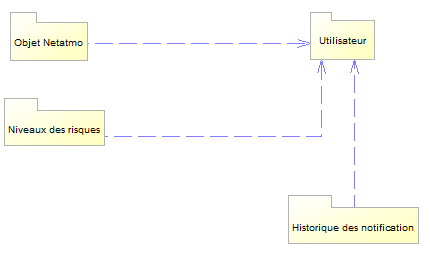
\includegraphics[width=0.64\textheight]{figures/pckg1}
	\end{center}
	\caption{Diagramme de paquetage}
	\label{fig3.3}
\end{figure}
\newpage
\subsection{Diagramme de classes}

\qquad Arrivant à ce stade nous allons décomposer chaque paquet du diagramme de la figure \ref{fig3.3} en diagramme de classes représentant ainsi les relations existante entre les classes de notre projet. Les relation entre les paquets sont représentées par les relations des classes qui les composent. Chaque classe est illustrée par ses attributs et les relations qui la relie aux classes de son paquet parent et des classes des autres paquets.

\subsubsection{Diagramme de classes relatif au paquet : Utilisateur}

\qquad Le diagramme de la figure \ref{fig3.4} représente le modèle des classes du paquet : Utilisateur.

\begin{figure}[!h]
	\begin{center}
		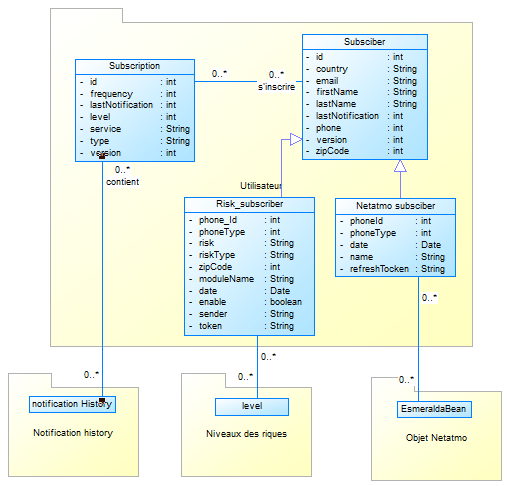
\includegraphics[width=0.64\textheight]{figures/pckg2}
	\end{center}
	\caption{Diagramme de classes relatif au paquet : Utilisateur}
	\label{fig3.4}
\end{figure}
\newpage
\subsubsection{Diagramme de classes relatif au paquet : Niveau des risques}

\qquad Ci-après est représenté la décomposition du paquet Niveau des risques. La figure \ref{fig3.5} illustre les classes membres du paquet : Niveau des risques.

\begin{figure}[!h]
	\begin{center}
		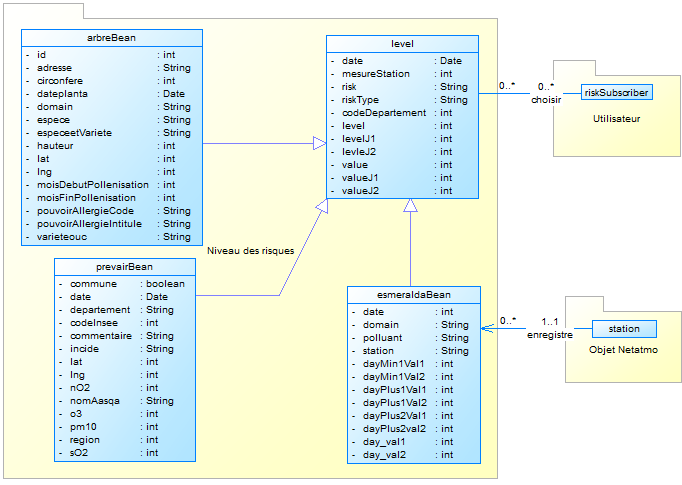
\includegraphics[width=0.64\textheight]{figures/pckg3}
	\end{center}
	\caption{Diagramme de classes relatif au paquet : Niveau des risques}
	\label{fig3.5}
\end{figure}

\newpage
\subsubsection{Diagramme de classes relatif au paquet : Objet Netatmo}

\qquad La figure \ref{fig3.6} illustre le diagramme de classes relatives au paquetage « Objet Netatmo ».

\begin{figure}[!h]
	\begin{center}
		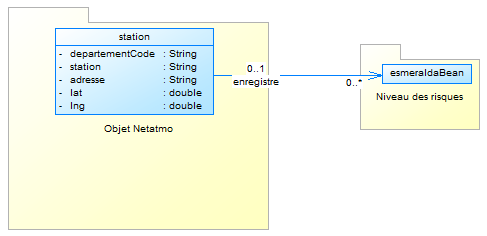
\includegraphics[width=0.64\textheight]{figures/pckg4}
	\end{center}
	\caption{Diagramme de classes relatif au paquet : Objet Netatmo}
	\label{fig3.6}
\end{figure}

\subsubsection{Diagramme de classes relatif au paquet : Historique des notifications}
\qquad Les classes du paquetage « Historique des notifications » sont modélisées dans la figure ci-dessous.

\begin{figure}[!h]
	\begin{center}
		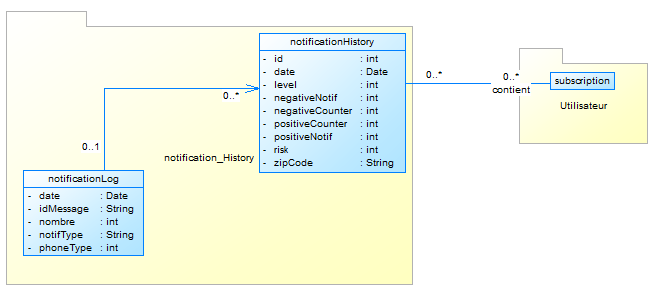
\includegraphics[width=0.64\textheight]{figures/pckg5}
	\end{center}
	\caption{Diagramme de classes relatif au paquet : Historique des notifications}
	\label{fig3.7}
\end{figure}

\subsection{Digrammes de séquence}
\qquad Les diagrammes de séquences permettent de donner une vue dynamique sur l’interaction entre l’acteur et le système. Nous représentons, dans cette section, des enchaînements de quelques scénarios à travers les diagrammes de séquences d’UML.

\subsubsection{Diagramme de séquence "Ajouter astuce"}

\qquad La figure \ref{fig3.8} illustre le diagramme de séquence de la fonctionnalité "Ajouter astuce" dont l'acteur est l'utilisateur et la post-condition est l'ajout d'une astuce. L'ajout d'une astuce se fait à plusieurs étapes. Après avoir accéder à la page d'ajout l'utilisateur interagira avec l'IHM contenant les champs à remplir pour accomplir la tache. Il saisira l'astuce, ses cordonnées (Pseudonyme et mail) et choisira le type de risque. Une fois les champs remplis, il peut confirmer son ajout en appuyant sur le bouton "submit" qui actionnera toute la chaine d'exécution expliquée par le tableau \ref{tab3.1}.


\begin{figure}
	\begin{center}
		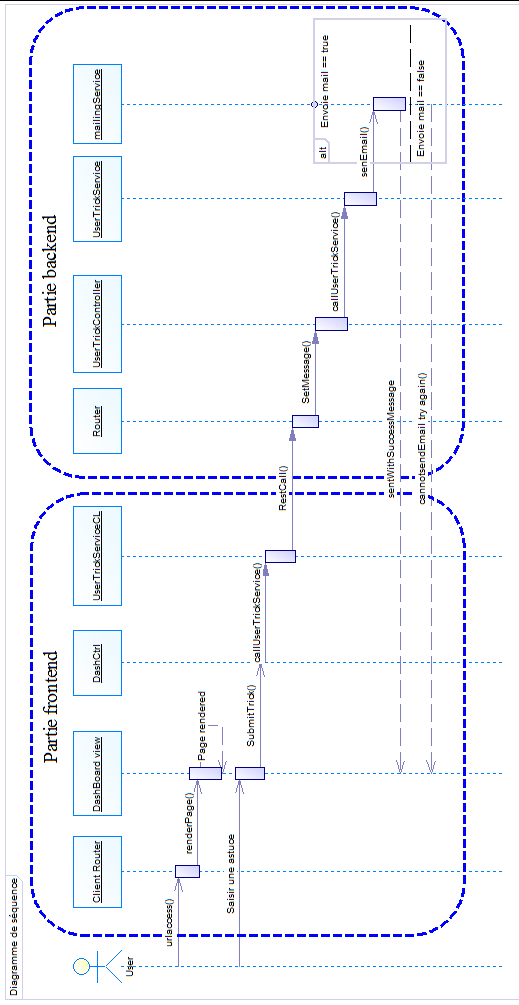
\includegraphics[height=\textheight]{figures/ds1}
	\end{center}
	\caption{Diagramme de séquence "Ajouter astuce"}
	\label{fig3.8}
\end{figure}

\newpage

\begin{table}
	\caption{Description textuelle de la chaine d'exécution de la fonctionnalité : Ajouter astuce}
	\label{tab3.1}
	\begin{center}
		\begin{tabular}{|L{2.2cm}|L{2.8cm}|L{2.8cm}|L{4.7cm}|}
			\hline
			\textbf{Fonction} & \textbf{Emplacement} & \textbf{Action/Fonction appelante} & \textbf{Rôle}\\
			\hline
			submitTrick & DashCtrl & Appui sur le bouton "Submit" & -Vérifie le contrôle sur les champs\\
			& & &-Appelle le UserTrickService\\
			\hline
			addUserTrick & UserTrickService & submitTrick & -Faire l'appel REST au serveur\\
			\hline
			setMessage & userTrickController & addUserTrick & -Appelle le service de constructionde message\\
			\hline
			buildMessage & userTrickService & setMessage & -Construire le message à envoyer pa mail\\
			\hline
			sendEmail & mailingServie & addUsertrick & -Envoyer l'astuce de l'utilisateur vers le mail de SmartData\\
			\hline
			
		\end{tabular}
	\end{center}
\end{table}

\subsubsection{Diagramme de séquence "Télécharger Rapport XLS"}

L'acteur de cette fonctionnalité est l'administrateur. $\grave{A}$ travers ce cas d'utilisation, l'administrateur peut télécharger un rapport sous format .xls de l'état de l'application. Après avoir accéder à l'URI correspondante, une IHM sera affichée qui à travers laquelle peut consulter le rapport sur le Web ou le télécharger en format .xls.

\begin{figure}[!h]
	\begin{center}
		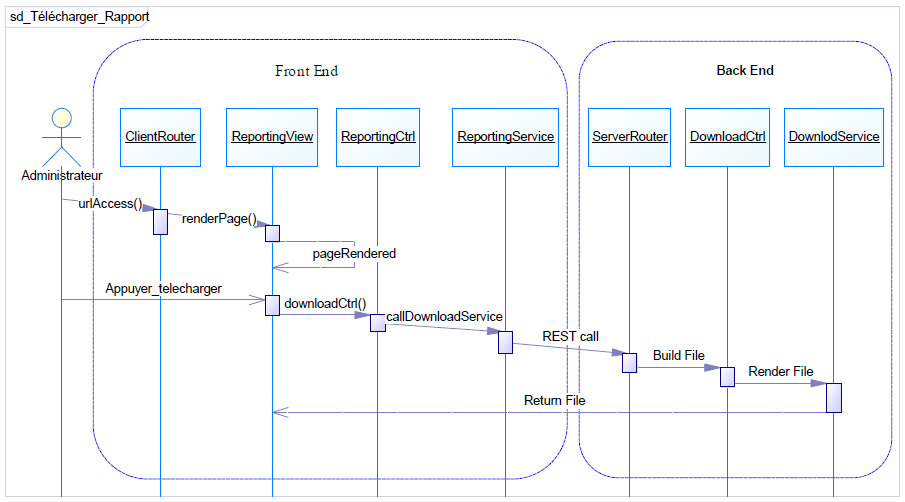
\includegraphics[width=0.64\textheight]{figures/sd2}
	\end{center}
	\caption{Diagramme de séquence "Télécharger Rapport XLS"}
	\label{fig3.9}
\end{figure}

\subsection{Diagramme d'activité}

\qquad Dans cette partie nous présentons, par le modèle du diagramme d'activité, les décisions prises par le système lors de l'exécution de la fonctionnalité "Ajouter Astuce". Nous nous intéressons aux diagrammes comportementaux d’UML. Les
diagrammes d’activités sont utilisés pour modéliser un workflow dans un use case ou entre plusieurs uses cases et pour spécifier une opération ( logique d’une opération ).\\

Le diagramme d’activité est le plus approprié pour modéliser la dynamique d’une tâche ou d’un use case. Nous commençons par montrer le diagramme d’activités relatives aux processus d’authentification et d’inscription puis celles qui sont relatives au processus d’ajout d’un membre.\\

La figure \ref{fig3.10} représente le diagramme d'activité du cas d'utilisation " Ajouter astuce ".

\begin{figure}[!h]
	\begin{center}
		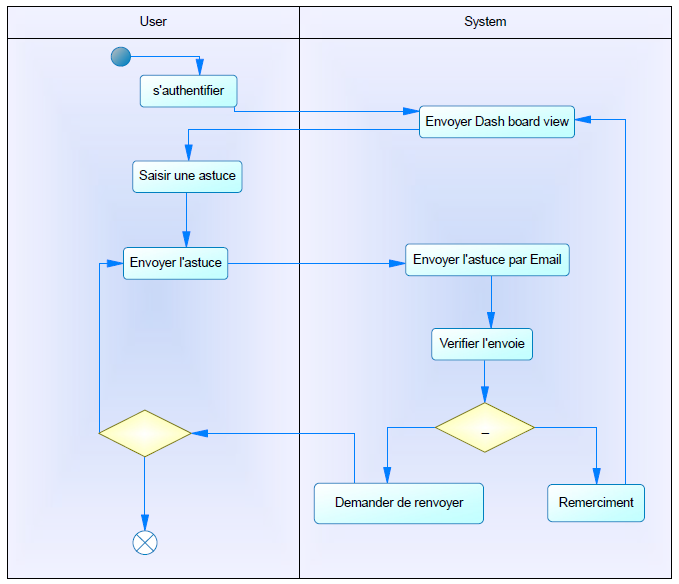
\includegraphics[width=0.64\textheight]{figures/ad1}
	\end{center}
	\caption{Diagramme d'activité du cas d'utilisation " Ajouter astuce "}
	\label{fig3.10}
\end{figure}

\subsection{Diagramme de déploiement} \label{para}

\qquad Un diagramme de déploiement est un diagramme UML qui fournit une représentation graphique de la configuration physique des éléments d'exécution de notre système. En phase de production, l'infrastructure physique nécessaire se compose de quatre parties majeures: 

\begin{itemize}
	\item Le Système de Gestion de Base de Données (SGBD)
	\item Le serveur Web pour la gestion des requêtes, des transactions vers la base de données et le lancement des Batch
	\item L'infrastructure Cloud pour l'exécution des Batch
	\item Les parties clientes : client mobile et client léger qui consomment les API REST de la partie Backend déployée dans le serveur Web.\\
\end{itemize}

La figure \ref{fig3.11} représente les différentes relations entre les parties du système déployés sur l'infrastructure physique ainsi que les protocoles utilisés pour assurer la communication entre les composantes de la configuration.

\begin{figure}[!h]
	\begin{center}
		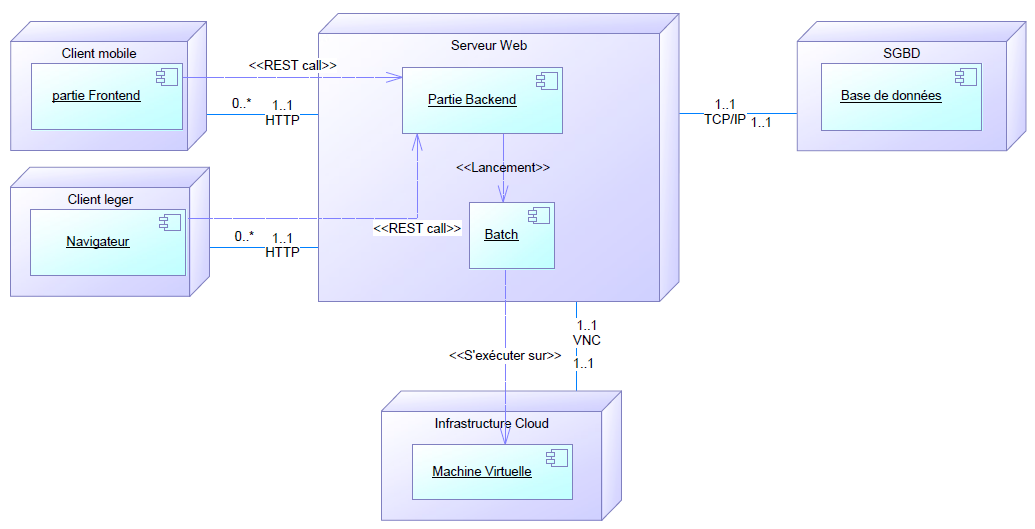
\includegraphics[width=0.63\textheight]{figures/dep}
	\end{center}
	\caption{Diagramme de déploiement}
	\label{fig3.11}
\end{figure}

\section*{Conclusion}

\qquad Nous avons traité dans ce chapitre l’étude conceptuelle de notre système. Nous avons présenté, dans un premier lieu, l’architecture globale de notre application. Puis, nous avons décrit plus en détails les différentes parties du système. Nous entamons à présent la partie relative à la réalisation de notre application.
	\chapter{Réalisation}

\section*{Introduction}
 \qquad Une fois nous avons fixé les grandes lignes de notre application et les pilonnes conceptuelles sur les niveaux global et détaillé nous pouvons passer à l'implémentation des modèles théoriques. Pour ce faire, nous allons choisir l'environnement de développement ainsi que les technologies nécessaires. Nous passons à la fin de ce chapitre à la présentation de quelques scénarios d'exécution à travers les interfaces Homme/Machine.
 
 \section{Environnement de travail}
 
\qquad Cette partie s'intéresse à l'environnement logiciel et matériel avec lequel nous avons mené notre projet.  

\subsection{Environnement physique}

\qquad Nous présentons dans ce paragraphe les équipements utilisés durant toutes les phases du projet : Développement, Débogage et Test unitaire. Le tableau \ref{tab4.1} présente la fiche technique des appareils utilisés.

\begin{table}[!h]
	\caption{Fiche technique des équipements utilisés}
	\label{tab4.1}
	\begin{center}
		\begin{tabular}{|L{5cm}|L{5cm}|}
			\hline
			\textbf{Ordinateur} & \textbf{Smartphone}\\
			- Modèle: Asus & - Modèle: Samsung Galaxy S5\\
			- Processeur: Intel i7 & - Processeur: Quad-core 2.5 GHz Krait 400\\
			- Mémoire: 12 GB RAM & - Mémoire: 2 GB RAM\\
			- Stockage interne: 1TB HDD & - Stockage interne: 16 GB\\
			- SE: WINDOWS 10  & - SE: Android 4.4.2\\
			\hline			
		\end{tabular}
	\end{center}
\end{table} 
\newpage
\subsection{Environnement logiciel}

\qquad Après la spécification des environnements physiques nécessaires à la réalisation, nous pouvons passer au choix de l'environnement logiciel. Les différents outils logiciels utilisés durant le stage pour la réalisation des fonctionnalités et la rédaction du rapport sont listés ci-après: 

\begin{itemize}
	\item \textbf{Eclipse}: Environnement de développement intégré (EDI) destiné principalement au développeur JAVA mais il est extensible vers d'autres langages tels que C/C++, PHP et plein d'autres. Nous pouvons combiner plusieurs langages sous un seul EDI à travers les plugins comme nous pouvons avoir un EDI pour chaque objectif. Nous avons utilisé Eclipse dans sa version destinée pour le Java Enterprise Edition durant le projet.
	
	\item \textbf{Visual Studio Code} : Éditeur de code source léger mais puissant qui fonctionne sur bureau et est disponible pour Windows, MacOS et Linux. Il est livré avec un support intégré pour JavaScript, TypeScript et Node.js et dispose d'un riche écosystème d'extensions pour d'autres langues (C ++, C \#, Python, PHP, Go).
	
	\item \textbf{BitBucket} : Gestionnaire de versions distribuées qui permet à une équipe de coopérer ensemble dans un projets large.
	
	\item \textbf{JIRA}: Gestionnaire de taches dans une équipe de travail. Il fournit un tableau de bord pour pouvoir gérer les story dans un environnement de développement SCRUM.
	
	\item \textbf{Confluence}: Logiciel de Wiki qui permet de rédiger la documentation sur le code source délivré.
	
	\item \textbf{PowAMC}: Environnement logiciel destiné à la conception UML. 
	
	\item \textbf{TeXStudio}: Éditeur de texte pour la rédaction des documents en Latex.
\end{itemize}

\section{Choix technologiques}

\qquad Cette partie s'intéresse aux choix des technologies et langages de programmation que nous allons utiliser pour parvenir à la finalité de notre projet comme le montre la figure \ref{fig4.1}.

\begin{figure}[!h]
	\begin{center}
		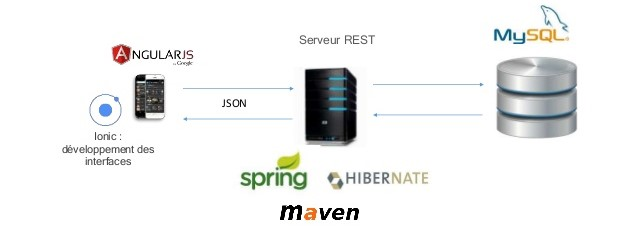
\includegraphics[width=0.64\textheight]{figures/archi}
	\end{center}
	\caption{Technologies utilisées}
	\label{fig4.1}
\end{figure}
\newpage
\begin{itemize}
	\item \textbf{HTML} : langage de balisage crée et utilisé pour écrire les pages Web.
	\item \textbf{CSS} : langage permettent de définir des règles appliquées à un ou plusieurs documents.
	\item \textbf{AngularJS} : Frame-work Javascript open-source, développé par Google, permettant de réaliser des applications Web dynamique en utilisant le modèle MV-VM (Model-View View-Model).
	\begin{itemize}
		\item \textbf{AngularUI Router} : Framework AnguarJS permettant de rajouter un router à la single page application en utilisant des vues imbriquées.
	\end{itemize}
	\item \textbf{Ionic} : Frame-work de développement d'applications hybrides. Ce frame-work permet de développer des applications mobiles pour divers différents environnements d'appareils téléphoniques (Android, Ios et WindowsPhone) en combinant à la fois les technologies Web (HTML, CSS et JavaScript) et les technologies de développement natives des différents environnements (Java SDK, Swift, Objective C ...)\cite{3}.
	\item \textbf{Java Enterprise Edition} : Extension du Java SE contenant des bibliothèques destinée au développement des applications Web robustes.
	\begin{itemize}
		\item \textbf{Jax-RS} : Spécification standard JEE qui fournit les méthodes du protocole HTTP pour pouvoir effectuer des appels REST. Ce standard est indépendant du format des données et est basé sur les POJO.
		\item \textbf{JPA} : API qui permet le mapping relationnel des objets Java sur les classes persistantes de la base de données, utilisé pour interroger la base lors des transactions faites par soit les utilisateurs soit par l'administrateur\cite{6}.
		\item \textbf{JDBC} : Bibliothèque qui permet l'accès au driver de la base de données. Cette bibliothèque est utilisée majoritairement dans les transactions faites lors des traitements par lots (Batch) car elle présente une légèreté de lors de l'interrogation de la base des données.
		\item \textbf{Spring Batch} : Premier Framework Java pour les traitements par lots. La framewrk offre un type par défaut de traitement Batch appelé Job où le job est composé de trois step: Read, Process et Write. Un autre type offert par la framework appelé tasklet offre la possiblité de personnaliser le traitement et d'ajouter autant d'étape que l'on veut à un traitement Batch. Nous avons opté pour le deuxième type parce que la plupart des traitements par lots de notre projet ne présente pas des étapes de lecture ni d'écriture \cite{4} (voir figure \ref{fig4.2}).
		\item \textbf{Apache POI}: Bibliothèque permettant de créer des fichiers Microsoft Office (XLS, Docx, PPT, ...)
		\item \textbf{StreamingOutput}: Bibliothèque permettant de télécharger (Donwnload) des fichier en streaming.  
		\item \textbf{Maven} : Gestionnaire de paquets pour l'environnement JEE.
	\end{itemize}  
	\item \textbf{MySQL} : Système de gestion de base de données relationnelles.
	\item \textbf{ServicesWeb REST} : Exposent entièrement les services comme un ensemble de ressources (URI) identifiables et accessibles par la syntaxe et la sémantique du protocole	HTTP
\end{itemize}

Ci-dessous est représenté un schéma descriptif des principales éléments qui constituent une application faisant appel à un traitement par lots. Généralement, l'architecture est réalisée en trois couches (voir figure \ref{fig4.2}):
\begin{itemize}
	\item Application mère ou couramment appelé projet parent qui contient tous les sous projets en particulier l'application Batch.
	\item Batch Core qui est la couche concernée par le lancement, la surveillance et la gestion des Batch.
	\item Batch infrastructure est la dernière couche qui fournit des API telles que la lecture, le processing et l'écriture des données.  
\end{itemize}
\begin{figure}[!h]
	\begin{center}
		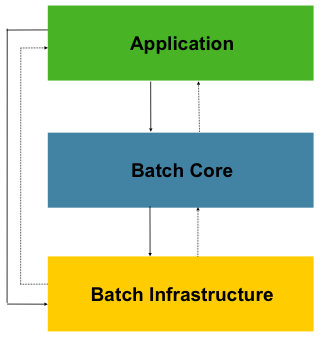
\includegraphics[height=4.5cm]{figures/batch_app}
	\end{center}
	\caption{Relation entre l'application serveur et les applications Batch}
	\label{fig4.2}
\end{figure}


\section{Scénarios d'exécution}

\qquad Ce paragraphe est consacré à la description de quelques scénarios d'exécution à travers les interfaces Homme/Machine fournies par l'application.

\subsection{Partie: Utilisateur}

\qquad L'utilisateur a un accès à l'application à travers une IHM sur son propre appareil téléphonique (smartphone). $\grave{A}$ l'entrée, l'application demande l'utilisateur de connecter son smartphone à Internet pour pouvoir récupérer les données du serveur comme l'indique l'interface \ref{fig4.3}.

\begin{figure}[!h]
	\begin{center}
 		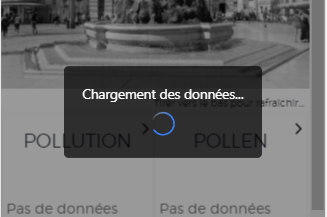
\includegraphics[width=7cm]{figures/Capture1}
 	\end{center}
 	\caption{Récupération des données}
 	\label{fig4.3}
\end{figure}
\newpage
Après avoir récupérer les données, l'application aura besoin de la région désirée. L'utilisateur peut alors, soit activer le service de géolocalisation, soit saisir le code ou le nom de la région comme le montre les exemples de la figure \ref{fig4.4}.

\begin{figure}[!h]
	\begin{center}
		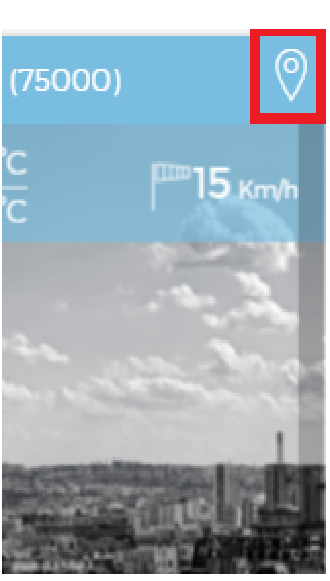
\includegraphics[width=5.25cm]{figures/gps}
		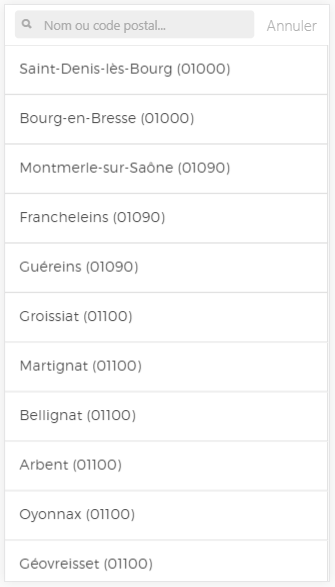
\includegraphics[width=5cm]{figures/choix_ville}
	\end{center}
	\caption{Indication de la ville : Par Service GPS / Par recherche}
	\label{fig4.4}
\end{figure}

Une fois l'application a pu se connecter à Internet et localiser l'utilisateur elle peut maintenant afficher les niveaux des risques auxquels l'utilisateur est abonné (voir figure \ref{fig4.5}).

\begin{figure}[!h]
	\begin{center}
		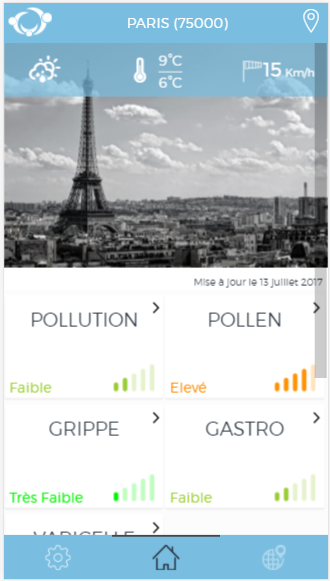
\includegraphics[width=4.6cm]{figures/dash_board}
	\end{center}
	\caption{Consultation des niveaux des risques}
	\label{fig4.5}
\end{figure}
\newpage
L'utilisateur peut aussi consulter des détails et des conseils relatives aux risques (voir figure \ref{fig4.6}) en cliquant sur le risque désiré.

\begin{figure}[!h]
	\begin{center}
		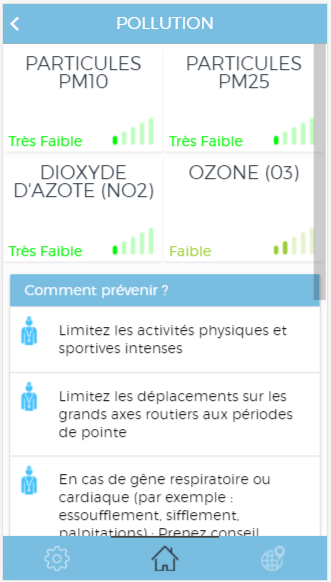
\includegraphics[width=5cm]{figures/detail_risk}
	\end{center}
	\caption{Consultation des détails et des conseils relatives à la pollution}
	\label{fig4.6}
\end{figure}

L'application offre encore la possibilité d'ajouter des astuces à l'application. Dans le menu principal, L'utilisateur peut faire descendre l'écran vers le bas, il trouvera alors la section intitulée "pense bête" où est affiché un message aléatoire relatif au risque ayant le plus haut niveau (voir figure \ref{fig4.7}).

\begin{figure}[!h]
	\begin{center}
		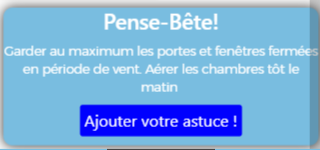
\includegraphics[width=7cm]{figures/pense_bete}
	\end{center}
	\caption{Section: Pense Bête}
	\label{fig4.7}
\end{figure}
\vspace{1cm}
En cliquant sur le bouton "Ajouter votre astuce", une popup s'affiche, comme le montre la figure \ref{fig4.8}, donnant ainsi la possibilité de remplir les informations qui concernent l'astuce ajoutée (Pseudonyme du contributeur, Adresse mail, Type de risque et Texte de l'astuce).

\begin{figure}[!h]
	\begin{center}
		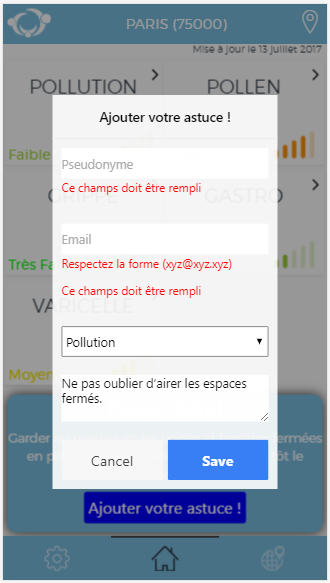
\includegraphics[height=8cm]{figures/ajout_trick}
	\end{center}
	\caption{Popup: Ajout d'astuces}
	\label{fig4.8}
\end{figure}
\newpage
La figure \ref{fig4.8} montre aussi le cas échéant où l'utilisateur saisit incorrectement les informations demandées. Au cas où les informations sont absentes ou incorrectes, un message d'erreur est affiché sous chaque champ erroné.

\vspace{0.5cm}

$\grave{A}$ la réception d'une notification, l'application navigue vers une interface où l'utilisateur peut choisir parmi trois conseils qui lui seront envoyé à chaque pique de niveau du risque en question. En cliquant sur le bouton "Enregistrer", il enregistre ses choix et retourne vers le menu principal (voir figure \ref{fig4.9}).

\begin{figure}[!h]
	\begin{center}
		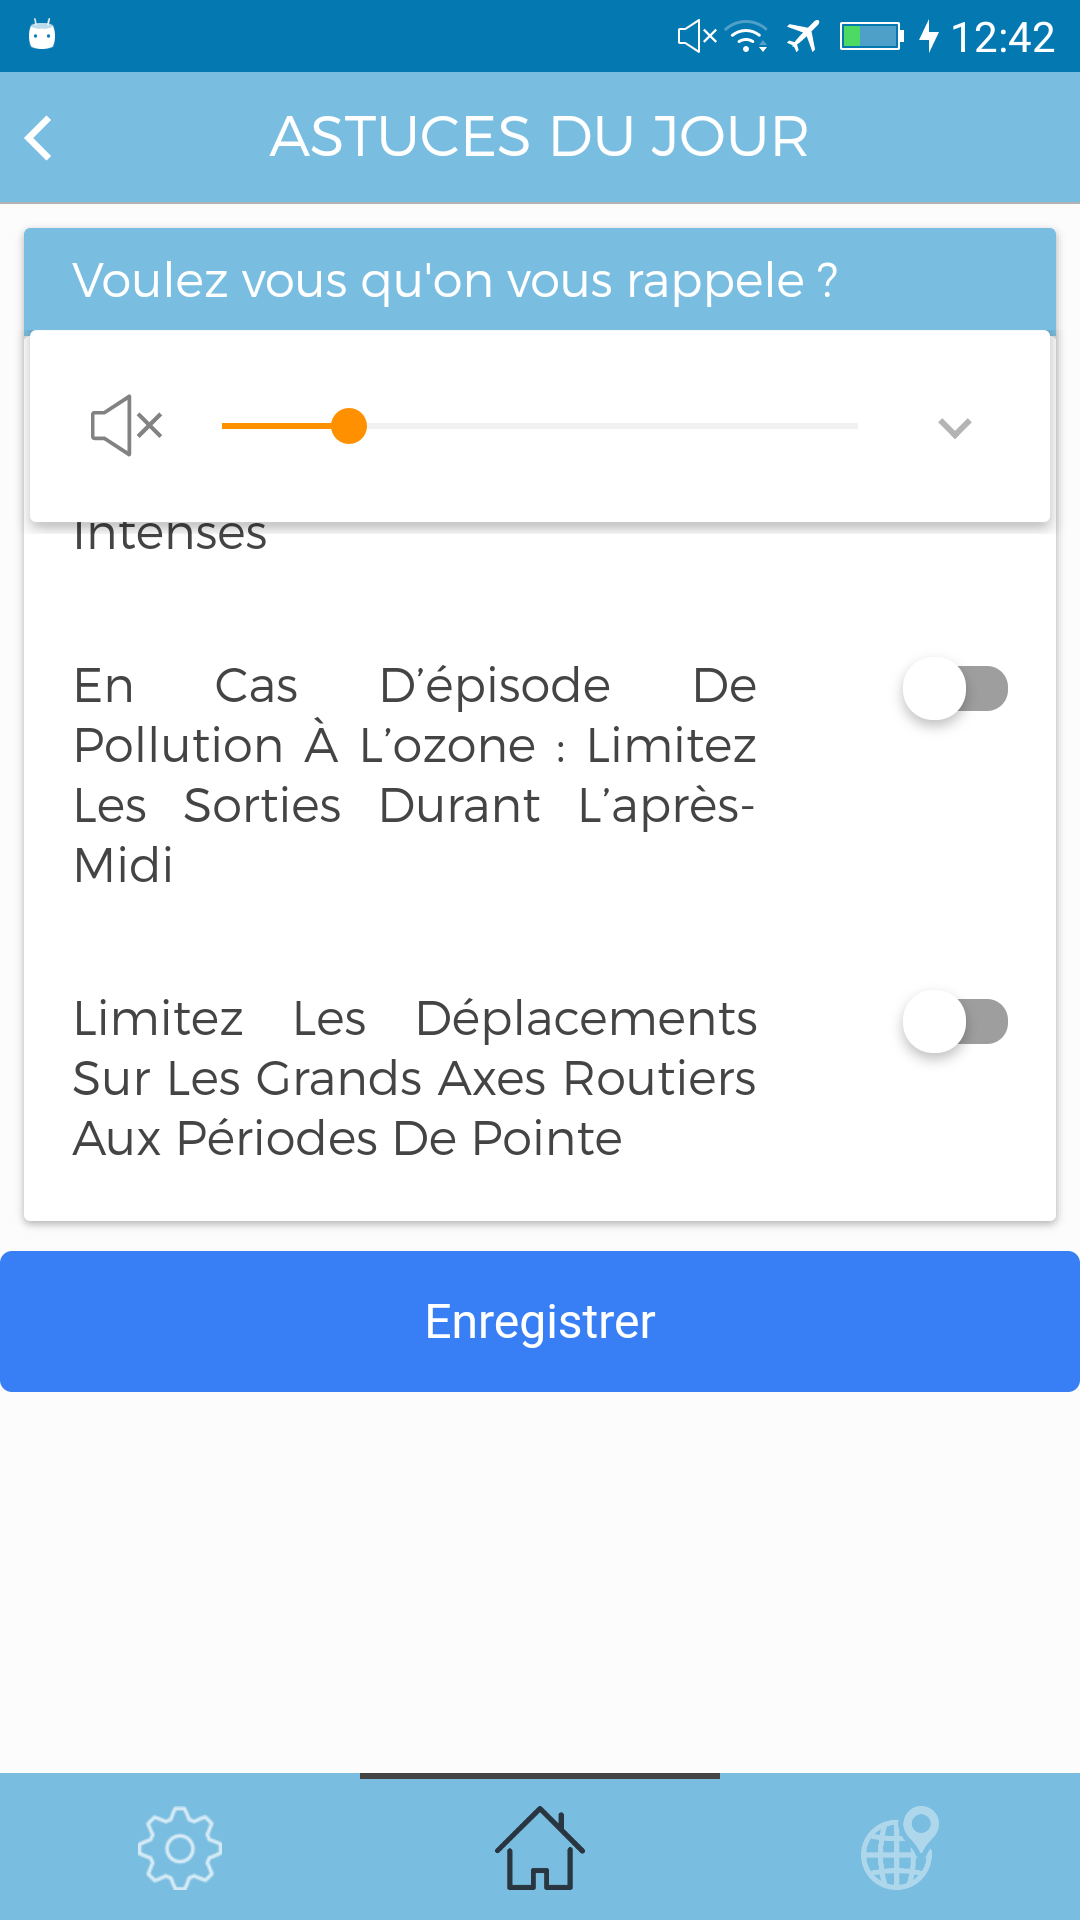
\includegraphics[height=8cm]{figures/rappel_trick}
	\end{center}
	\caption{Choix des astuces "Pique des niveaux des risques"}
	\label{fig4.9}
\end{figure}

 L'utilisateur consulte la rubrique configuration pour paramétrer l'application (voir figure \ref{fig4.10}). Cette dernière accorde à l'utilisateur plusieurs fonctionnalités: 
\begin{itemize}
	\item S'abonner et/ou se désabonner d'un risque
	\item Permettre l'accès aux données personnelles (position géographique)
	\item S'abonner ou se désabonner aux notifications
\end{itemize} 

\begin{figure}[!h]
	\begin{center}
		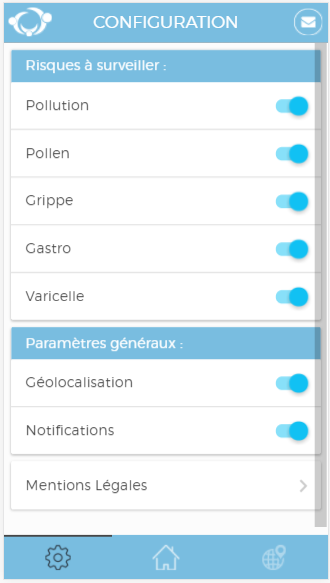
\includegraphics[height=7cm]{figures/subscribe}
	\end{center}
	\caption{Interface Configuration}
	\label{fig4.10}
\end{figure}

Finalement, l'utilisateur peut utiliser les boutons de navigation en bas de l'écran pour consulter les différentes interfaces.Il peut alors solliciter les stations de mesure affichées sur la carte géographique avec le niveau des risques. Il a aussi la possibilité de balayer les risques et les villes. La figure \ref{fig4.11} illustre la rubrique Carte des risques.
\begin{figure}[!h]
	\begin{center}
		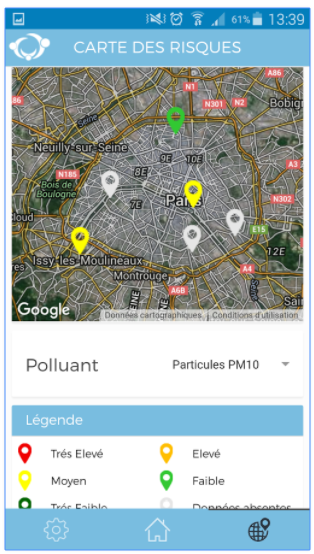
\includegraphics[height=7cm]{figures/station}
	\end{center}
	\caption{Interface Carte des risques}
	\label{fig4.11}
\end{figure}
 
\subsection{Partie: Administrateur}

\qquad L'administrateur a accès à une interface pour visualiser le rapport journalier de l'application. Les informations affichées sont: 
\begin{itemize}
	\item L'historique des notifications
	\item Les villes les plus actives
	\item Les risques les plus consultés
\end{itemize}

L'administrateur peut également télécharger une version xls pour une éventuelle utilisation hors ligne, en cliquant sur le bouton "Export". Le serveur prépare un fichier xls contenant les informations actualisées du rapport, ensuite l'envoie vers la machine de l'administrateur.
La figure \ref{fig4.12} montre l'interface affichée à l'administrateur.

\begin{figure}[!h]
	\begin{center}
		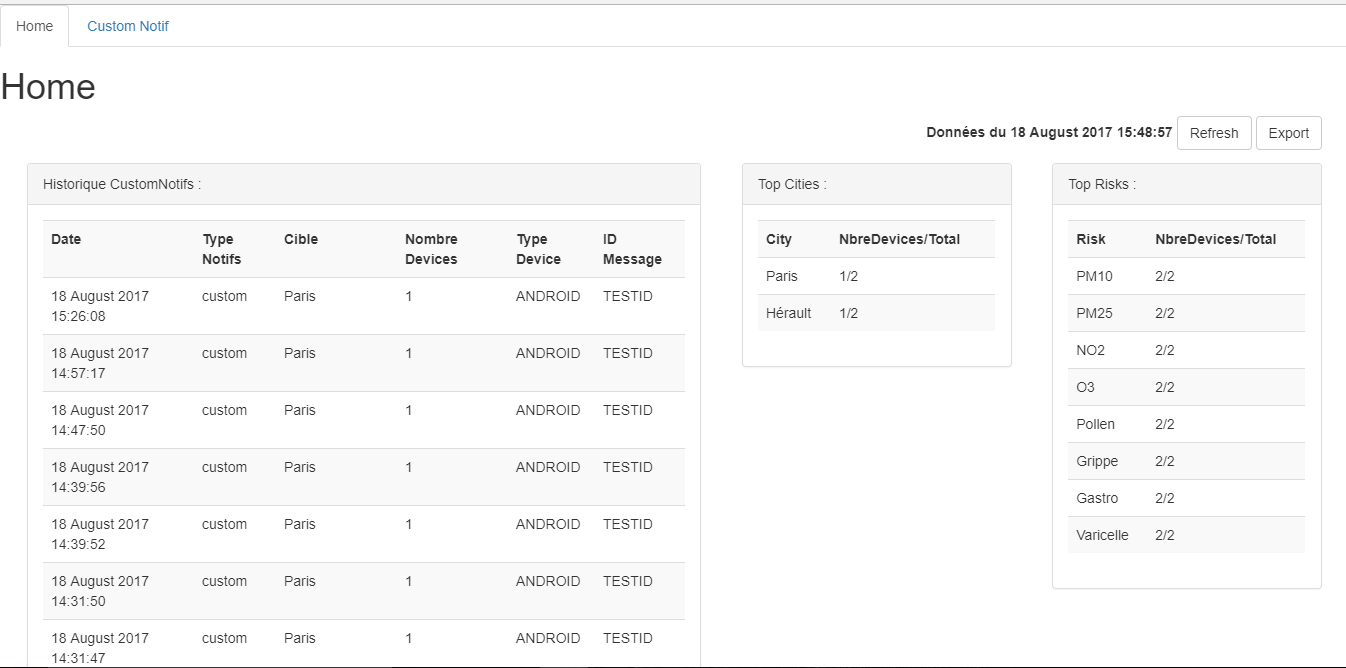
\includegraphics[height=7cm]{figures/admin}
	\end{center}
	\caption{Interface Administration}
	\label{fig4.12}
\end{figure}

L'administrateur peut aussi envoyer des notifications personnaliser aux utilisateurs (voir figure \ref{fig4.13}).

\begin{figure}[!h]
	\begin{center}
		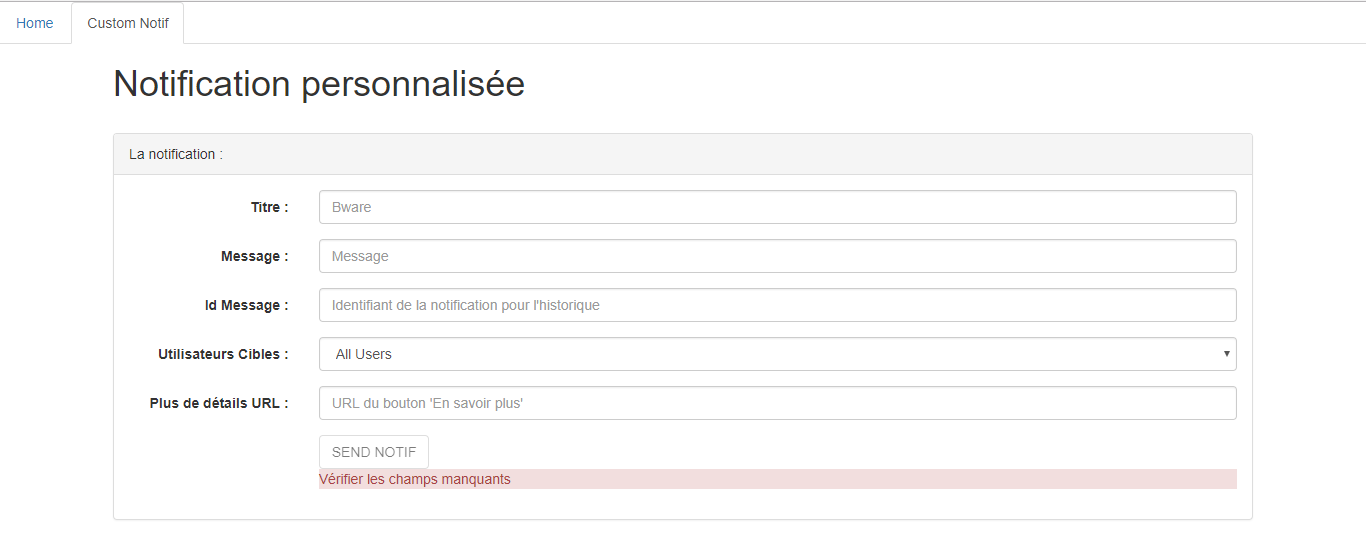
\includegraphics[height=5.5cm]{figures/notif}
	\end{center}
	\caption{Interface Notification personnalisée}
	\label{fig4.13}
\end{figure}

\section{Déploiement et publication de l'application}

\subsection{Déploiement de la partie serveur}
\qquad Les étapes décrites ci-dessous concernent le déploiement en phase de pré-production. Avant de déployer la partie backend dans la machine distante, il faut impérativement préparer le projet à être exécuté dans le nouvel environnement. La différence entre la phase débeugage et la phase production réside majoritairement dans les ressources. Dans la phase débeugage, le serveur Web, le SGBD et l'application cliente existent tous dans la machine du développeur par contre dans la phase pré-production on va séparer chacune de ces parties dans une machine à part comme il est indiqué dans le paragraphe \ref{para}. Cette séparation est effectuée dans le but de tester l'architecture complète avant de la faire passer vers le client final. Pour déployer la partie serveur il faut alors effectuer les étapes suivantes:
\begin{itemize}
	\item Reconfigurer l'application avec les nouvelles adresses et ports utilisés en pré-production (Base de donnée, ports ouverts de l'application...)
	\item Préparer l'application à être exécuté dans le nouvel environnement (Variables d'environnement, variable système...)
	\item Se connecter en Secure Shell (SSH) à la machine distante par la commande
	\begin{itemize}
		\item ssh root@<Adresse IP de la machine>
	\end{itemize}
	\item Éteindre le serveur Web
	\begin{itemize}
		\item /usr/share/tomcat8/bin/shutdown.sh
	\end{itemize}
	\item Supprimer le backup existant et le remplacer par un backup de la version en cours
	\begin{itemize}
		\item rm -rf webapps-smartdata.old
		\item cp -rf webapps-smartdata webapps-smartdata.old
	\end{itemize}
	\item Copier le Web Archive (WAR) vers la machine en utilisant le protocole Secure Copy (SCP) et le placer dans le serveur Tomcat
	\begin{itemize}
		\item scp sd.war root@<Adresse IP de la machine>:/root/documents/2017-07-26
		\item cp /root/document/2017-07-26/sd.war /var/lib/tomcat8/webapps
	\end{itemize}
	\item Redémarrer le serveur Tomcat
	\begin{itemize}
		\item sudo service tomcat8 start; tail -f logs/catalina.out
	\end{itemize}   
\end{itemize} 

\subsection{Publication de l'application dans le play store}

\qquad Pour rendre accessible notre application aux utilisateurs il faut publier celle-ci dans les stores spécifiques à chaque système d'application mobile. Les étapes décrites ci-après concernent la publication dans le play store de Google spécifique à Android. Pour publier l'application mobile dans le store il faut:
\begin{itemize}
	\item Actualiser les informations de configuration de l'application (version, IP du serveur de production...)
	\item Générer une version release de l'application mobile
	\begin{itemize}
		\item ionic cordova build --release android
	\end{itemize}
	\item Générer une clé de signature (il faut l'utiliser pour toute les versions de l'application)
	\begin{itemize}
		\item keytool -genkey -v -keystore release-key.keystore -alias alias\_name -keyalg RSA -keysize 2048 -validity 10000
	\end{itemize}
	\item Signer le binaire avec la clé de signature
	\begin{itemize}
		\item jarsigner -verbose -sigalg SHA1withRSA -digestalg SHA1 -keystore release-key.keystore binary-unsigned.apk alias\_name
	\end{itemize}
	\item Ziper le binaire
	\begin{itemize}
		\item zipalign -v 4 binary-unsigned.apk ready.apk
	\end{itemize}
	\item Télécharger le binaire vers le play store
	\item Publier le binaire dans la forme désirée (Alpha, Beta, Production)
\end{itemize}

\section*{Conclusion}
\qquad Dans ce chapitre, nous avons présenté l’environnement logiciel et matériel dans lequel notre projet a été élaboré. Nous avons ensuite, présenté notre travail à travers un enchaînement de quelques scénarios d’exécution illustrés par des interfaces de l’application. Finalement, nous avons présenté les étapes nécessaires pour déployer notre projet et publier l'application mobile.

	\addcontentsline{toc}{chapter}{Conclusion générale}
\chapter*{Conclusion générale}

\qquad Tout au long du projet nous étions menés à concevoir et à apporter des améliorations à une application mobile permettant de suivre le niveau de pollution de l'air. L’application facilitera aux utilisateurs le suivie de l'état quotidien de l'air. Elle permet aussi à l'administrateur de suivre l'état de l'application à travers des rapports à jour sous format xls qu'il peut télécharger.\\

Ce rapport décrit toutes les phases de la réalisation du projet. Commençant par le contexte général puis la présentation de l’objectif du projet ainsi qu’une étude menée sur les solutions existantes sur le marché de l'e-santé et les limites des solutions proposées. Ensuite nous avons passé à l’analyse des besoins fonctionnels et non-fonctionnels ce qui nous a permis de fixer le cahier des charges auquel doit répondre notre application. Ce qui nous a permis d’aborder la partie de la conception où nous avons spécifié l’architecture de notre projet et ses composantes. Enfin nous avons précisé l’environnement où nous avons réalisé notre application et les outils technologiques utilisés tout au long de la phase du développement.\\

Le stage ingénieur nous a permis de consolider les connaissances acquises dans notre cursus académique, en nous donnant la possibilité d’appliquer les notions théoriques du cours qui nous ont été une base solide pour comprendre l’engin du développement mobile hybride multi-plateforme.\\

Notre application étant fonctionnelle, mais elle présente quelques imperfections. Nous projetons de lui rajouter un module qui permettra aux utilisateurs de s'interagir et de partager les informations sur les réseaux sociaux ce qui donnera plus de visibilité à l'application. Une majeure amélioration qui peut être additionnée consiste à un module de prévision des niveaux des risques à travers des algorithmes de Machine Learning et d'Intelligence Artificiel. 
	
\begin{thebibliography}{9}
	\bibitem{bib0}
	Communiqué de presse OMS: URL: http://www.who.int/mediacentre/news/releases/2016/air-pollution-estimates/fr/(visité le 10/09/2017)
	
	\bibitem{bib1}
	Guide de démarrage Scrum: URL: http://www.agiliste.fr/guide-de-demarrage-scrum/(visité le 03/09/2017)
	
	\bibitem{bib2}
	Documentation Ionic: URL: http://ionicframework.com/ (visité le 15/09/2017)
	
	\bibitem{bib3}
	Lucas Ward, Dave Syer, Thomas
	Risberg, Robert Kasanicky, Dan Garrette, Wayne Lund,
	\emph Spring Batch - Reference Documentation, 2009
	
	\bibitem{bib4}
 	ARNAUD COGOLUEGNES, THIERRY TEMPLIER, GARY GREGORY,	OLIVIER BAZOUD,
	\emph Spring Batch in Action, 2012
	
	\bibitem{bib5}
	Oliver Gierke, Thomas Darimont, Christoph Strobl, Mark Paluch,
	\emph Spring Data JPA - Reference Documentation, avril 2017
		
	\bibitem{bib6}
	Jon Brisbin, Oliver Gierke, Greg Turnquist,
	\emph Spring Data REST - Reference Documentation, avril 2017
	
	\bibitem{bib7}
	Salah BENNOUR,
	\emph Tutoriel Ionic framework, 2015
	
	
	
\end{thebibliography}
	\addcontentsline{toc}{part}{Bibliographie}
	%Ne pas numéroter cette partie
\part*{Annexes}
%Rajouter la ligne "Annexes" dans le sommaire
\addcontentsline{toc}{part}{Annexes}

\chapter*{Annexe 1
\\RESTful Web Services}
\addcontentsline{toc}{chapter}{Annexe 1}
\makeatletter
\renewcommand{\thesection}{\@arabic\c@section}
\makeatother
\renewcommand\thefigure{\thesection.\arabic{figure}}    
\setcounter{figure}{0}

\renewcommand\thetable{\thesection.\arabic{table}}    
\setcounter{table}{0}
%recommencer la numérotation des section à "1"
\setcounter{section}{0}

\qquad Representational State Transfer ou communément REST est une architecture d'application basée sur le standard HTTP. REST utilise les opérations natives de HTTP : POST, GET, PUT, DELETE pour le mapping sur les quatre fonctions fondamentales d'une base de données qui sont Create, Read, Delete, et Update. Ces services peuvent ensuite être consommés par des clients authentifiés \cite{7}.\\

Les services Web REST sont utilisés pour développer des applications orientées ressources dans lesquelles chaque composant est une ressource accessible en utilisant les méthodes standards du HTTP. Les applications qui respectent les architectures orientées ressources sont appelées RESTful.

\section{Caractéristiques}

\begin{itemize}
	\item Sans état : le serveur ignore l'état des clients entre les requêtes
	\item Cacheable : les candidats doivent être capables de garder en mémoires des informations.
	\item Orienté clients serveur : le client et le serveur sont les entités communiquent dans une architecture REST. Le client requière une ressource et le serveur la lui fournira, s'il est authentifié.
	\item Réalisé en couche : le pattern MVC doit être respecté.
	\item Les ressources sont accessibles à travers les méthodes du HTTP (POST, GET, PUT, DELETE)\\
\end{itemize}

La communication entre le serveur et les clients peut se faire sous plusieurs formats : JASON, XML, CSV... Le présent projet utilise le format JSON pour la communication client-serveur.

\section{Méthodes du HTTP}

\begin{itemize}
	\item GET Accès en lecture seule à la ressource,
	\item PUT Création d’une nouvelle ressource,
	\item DELETE Suppression d’une ressource,
	\item POST Création d’une nouvelle ressource ou mise à jour d’une ressource existante
\end{itemize}

\begin{table}[!h]
	\caption{Exemple d’une API REST}
	\begin{tabular}{|L{3cm}|L{3cm}|L{4cm}|L{3cm}|}
		\hline
		Méthode HTTP & Route & Description & Type de l'opération\\
		\hline
		\hline
		GET & /Utilisateur/one & Obtenir un Utilisateur & lecture seule\\
		\hline
		GET & /Utilisateur/all & Obtenir tous les Utilisateurs & lecture seule\\
		\hline
		POST & /Utilisateur/add & Ajouter un Utilisateur & écriture seule\\
		\hline
		PUT & /Utilisateur/update & Mettre à jour un Utilisateur & écriture seule\\
		\hline
		DELETE & /Utilisateur/delete & Supprimer un Utilisateur & écriture\\
		\hline  
	\end{tabular}
	
\end{table}

\pagebreak

\section{Format de données}

Les différentes parties de notre application communiquent en utilisant le format de représentation de données JSON (JavaScript Object Notation – Notation Objet issue de JavaScript) qui est un format léger d'échange de données. Il est facile à lire ou à écrire pour des humains. 

JSON possède deux structures de données :
\begin{itemize}
	\item Objet : collection de pairs nom/valeur
	\item Liste : liste de valeurs ordonnés
\end{itemize}

la figure \ref{figB1} représente les deux structures de données JSON.\\

\begin{figure}[!h]
	\begin{center}
		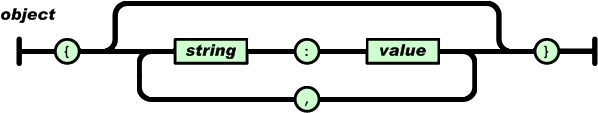
\includegraphics[width=14.7cm]{figures/object.png}
		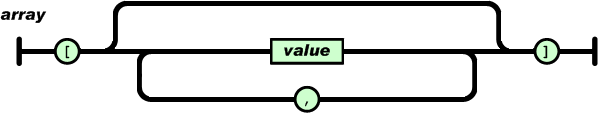
\includegraphics[width=14.7cm]{figures/array.png}
	\end{center}
\caption{Structures de données JSON}
%\source{Présentation de JSON\cite{bib12}}
\label{figB1}
\end{figure}
\newpage
\subsection{Exemple}
\textbf{paramètre de la requête d'un level :}

\begin{figure}[!h]
	\begin{center}
		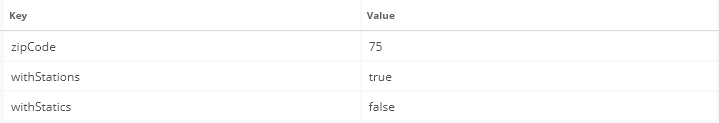
\includegraphics[width=14cm]{figures/param.png}
	\end{center}
	\caption{Paramètres d'une requête}
	\label{figB2}
\end{figure}

\textbf{Réponse du serveur :}

\begin{figure}[!h]
	\begin{center}
		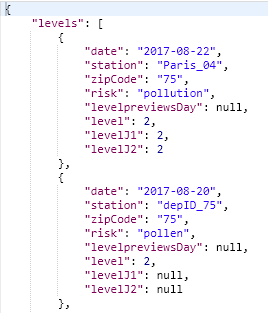
\includegraphics[width=6cm]{figures/reponse.png}
	\end{center}
	\caption{Réponse du serveur}
	\label{figB3}
\end{figure}

 

%\input{./annexes/annexe2.tex}

%\input{./annexes/annexe3.tex}


\end{document}